% p1_context_engineering.tex
% AI Agent 的核心技术：Context Engineering
% 编译方式: xelatex p1_context_engineering.tex

\documentclass[12pt,a4paper]{article}

% ============================================================
% 字体与中文支持
% ============================================================
\usepackage{fontspec}
\usepackage{xeCJK}
\setCJKmainfont[BoldFont=PingFang SC Semibold]{PingFang SC}
\setCJKsansfont[BoldFont=PingFang SC Semibold]{PingFang SC}
\setCJKmonofont{PingFang SC}
\setmainfont{Palatino}
\setsansfont{Helvetica Neue}
\setmonofont{Menlo}

% ============================================================
% 页面布局
% ============================================================
\usepackage[
  top=2.5cm,
  bottom=2.5cm,
  left=2.5cm,
  right=2.5cm
]{geometry}

% ============================================================
% 常用宏包
% ============================================================
\usepackage{amsmath,amssymb}
\usepackage{graphicx}
\graphicspath{{images/}}
\usepackage{longtable,booktabs,array}
\usepackage{enumitem}
\usepackage{xcolor}
\usepackage{hyperref}
\hypersetup{
  colorlinks=true,
  linkcolor=blue!70!black,
  urlcolor=blue!70!black,
  pdfauthor={整理自李宏毅老师 AI Agent 系列课程},
  pdftitle={AI Agent 的核心技术：Context Engineering},
}

% ============================================================
% 段落与间距
% ============================================================
\usepackage{parskip}
\setlength{\parindent}{0pt}
\setlength{\parskip}{6pt plus 2pt minus 1pt}

% ============================================================
% 引用环境美化
% ============================================================
\usepackage{mdframed}
\newmdenv[
  topline=false,
  bottomline=false,
  rightline=false,
  linewidth=3pt,
  linecolor=blue!40,
  innerleftmargin=12pt,
  innerrightmargin=12pt,
  innertopmargin=8pt,
  innerbottommargin=8pt,
  backgroundcolor=blue!3,
  skipabove=10pt,
  skipbelow=10pt,
]{myquote}

% ============================================================
% 节标题样式
% ============================================================
\usepackage{titlesec}
\titleformat{\section}{\Large\bfseries\sffamily}{}{0em}{}[\vspace{-0.5em}\rule{\textwidth}{0.5pt}]
\titleformat{\subsection}{\large\bfseries\sffamily}{}{0em}{}
\titleformat{\subsubsection}{\normalsize\bfseries\sffamily}{}{0em}{}
\setcounter{secnumdepth}{0}  % 不编号

% ============================================================
% 防止 overfull
% ============================================================
\setlength{\emergencystretch}{3em}
\tolerance=1000

% ============================================================
% 图片插入命令
% ============================================================
\newcommand{\keyslide}[2]{%
  \begin{figure}[htbp]
    \centering
    \includegraphics[width=0.92\textwidth]{#1}
    \caption{#2}
  \end{figure}
}

% ============================================================
\begin{document}

% ============================================================
% 标题页
% ============================================================
\begin{titlepage}
  \centering
  \vspace*{3cm}
  {\Huge\bfseries\sffamily AI Agent 的核心技术：\\[0.3em] Context Engineering\par}
  \vspace{1.5cm}
  {\Large 整理自李宏毅老师 AI Agent 系列课程第 1 集\par}
  \vspace{2cm}
  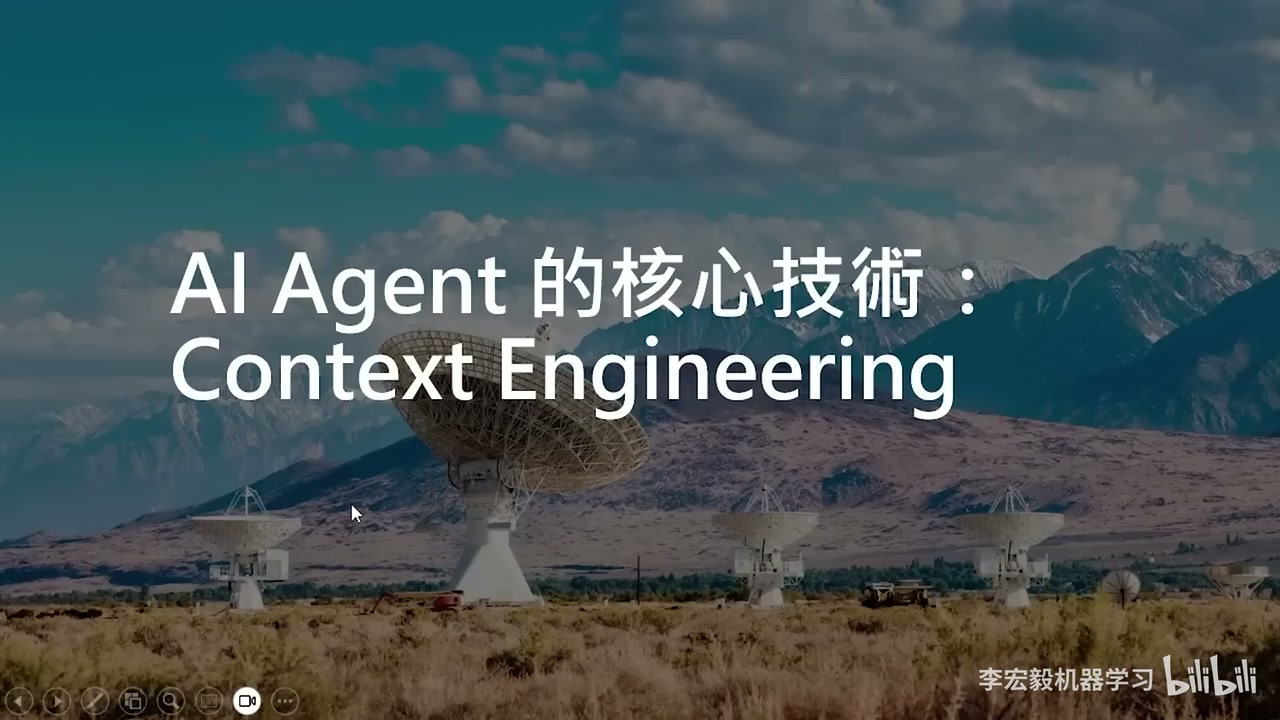
\includegraphics[width=0.8\textwidth]{p1_slide_0001.jpg}
  \vfill
  {\large \today\par}
\end{titlepage}

\newpage
\tableofcontents
\newpage

% ============================================================
\section{课程概览}
% ============================================================

本集课程分为三个部分：

\begin{enumerate}[leftmargin=2em]
  \item \textbf{AI Agent 背后的核心技术} —— 系统化讲解 Context Engineering
  \item \textbf{AI Agent 之间的互动}
  \item \textbf{AI Agent 对未来工作可能造成的冲击}
\end{enumerate}

本文聚焦于第一部分：Context Engineering。

% ============================================================
\section{一、为什么需要 Context Engineering？}
% ============================================================

\subsection{语言模型的本质：文字接龙}

语言模型的工作方式非常简单——你给它一个输入（Prompt），它就接一段话出来。人类给语言模型一个输入，语言模型给人类一个回应。这个回应不一定是一句话，它可能是一个"使用工具"的指令，这个指令会去驱动环境中的某个程序被执行，然后得到工具的输出。

\subsection{"活在当下"的语言模型}

当我们要把工具的输出传给语言模型时，\textbf{不能只给它工具的输出}。大家要记得：\textbf{语言模型是活在当下的}，它只看当前的输入，不管你之前给过它什么。

所以当你得到工具一的输出时，需要把之前人类给的命令、语言模型自己操控工具的指令、加上工具的输出，\textbf{全部拼接在一起}，一次性丢给语言模型。对语言模型来说，它看到的就是一串非常长的输入，然后再给一个回应。

同样的步骤反复下去——语言模型说它要使用工具二、工具三……每次都把之前发生的所有事情串成一串越来越长的输入，再丢给语言模型。

\subsection{难点：输入长度有限}

这里的核心问题是：\textbf{语言模型的输入长度是有限的}，它不能吃无限长的输入。

这就是为什么我们需要 AI Agent。AI Agent 就是横亘在语言模型与人类（或语言模型要执行的环境）之间的一个界面。它就像语言模型的"守门人"、语言模型的"经纪人"——\textbf{它决定语言模型会看到什么}。

来自外界的输入会经过 AI Agent 的筛选，语言模型真正看到的是 AI Agent 筛选过的、\textbf{长度合适}的输入——不能太长（超出上限），也不能太短（否则语言模型不知道之前发生了什么，无法正确做"接龙"）。

\begin{myquote}
AI Agent 帮语言模型管理它的输入，让输入的长度合适——这件事情就叫做 \textbf{Context Engineering}。
\end{myquote}

\begin{myquote}
\textbf{注意}：今天的 OpenCloud 只是 AI Agent 的一个初代例子。也许再过几年回头看 OpenCloud，就好像今天拿着 iPhone 去看过去的 Nokia 手机一样。我们现在看到的只是 AI Agent 的原型。
\end{myquote}

% ============================================================
\section{二、Context Engineering 的形式化描述}
% ============================================================

\subsection{没有 Context Engineering 的情况}

如果不做 Context Engineering，语言模型与外界的互动本质上就是一个 \textbf{for 循环}——从 step 1 到无限大：

\begin{itemize}[leftmargin=2em]
  \item 有一个初始输入 $I_1$（可以是一个非常 high level 的目标，比如"成为 YouTuber"）
  \item 用 $C$ 来表示当前所有环境中发生的事情（即 Context），初始时 $C$ 为空
  \item 每个循环中：把之前所有发生的事情 $C_t$ 加上当前输入 $I_t$ 拼接，丢给语言模型，得到输出 $O_t$
  \item 然后将 $I_t$ 和 $O_t$ 接到 $C_t$ 后面，更新为 $C_{t+1}$
\end{itemize}

\subsection{加入 Context Engineering}

唯一的改变就是\textbf{最后一步}：我们不再直接把输入和输出拼接到 Context 上，而是做一个更复杂的操作（用大写 $\mathbf{F}$ 表示）。这个 $F$ 把 Context、当前输入、当前输出，转换成新的 Context $C_{t+1}$。

\textbf{至于这个 $F$ 要做什么？这就是 Context Engineering，也就是 AI Agent 要做的事情。}

% ============================================================
\section{三、压缩：Context Engineering 的核心操作}
% ============================================================

之所以需要 Context Engineering，最核心的需求就是语言模型的输入不能太长。所以那个大 $F$ 里面，\textbf{最重要的功能就是压缩}——把本来很长的历史记录压短。

\keyslide{p1_slide_0010.jpg}{压缩的两种方式：LLM Summary vs Hard Clear}

\subsection{方式一：LLM Summary（用语言模型做摘要）}

把整个历史记录中（扣掉 System Prompt 的部分）比较久远的历史记录，通过某个语言模型生成摘要。原本很长的历史记录就变成了一段简短的摘要，再继续拼接上新的信息。

\subsection{方式二：Hard Clear（Observation Masking）}

更简单粗暴的方式：如果某一段文字原本是某个工具的输出（而工具输出往往非常长），就直接把那一段长篇大论改成 \textbf{"这里曾经有个工具的输出"} 就结束了。

这听起来可能很"烂"，但\textbf{这个方法还真的有用}。

\subsection{实验验证：SWE-Bench 上的对比}

有一篇探讨 \href{https://arxiv.org/abs/2508.21433}{Observation Masking} 的论文在 SWE-Bench（Software Engineering Benchmark，让语言模型去修复 GitHub Repo 中的 Issue）上做了对比实验：

\begin{itemize}[leftmargin=2em]
  \item \textbf{黑色点（Raw Agent）}：没有做任何压缩，所有环境信息通通堆进历史记录。虽然在多数情况下表现不错，但相较于其他方法，会耗费更多的 Token。
  \item \textbf{红色方块（LLM Summary）}：用语言模型对上下文进行压缩。与黑色点比起来差别不大，说明压缩是有效的。
  \item \textbf{三角形（Observation Masking）}：直接把工具输出换成"这里曾经有个工具的输出"。\textbf{表现与 LLM Summary 差不多！}
\end{itemize}

也就是说，与其花钱去调用一个语言模型做摘要，不如直接把工具输出替换成一句话，效果差不多。

\subsection{"轨迹延长"现象}

有一个有趣的例外：在某些情况下，做了压缩反而\textbf{没有比较省钱}。原因是——当你做压缩后，上下文虽然变短了，但因为一些步骤信息丢失了，语言模型会觉得"我刚才到底执行过这个工具了吗？还没有吗？"于是\textbf{重复做了已经做过的事}，导致执行步骤变多，总 Token 消耗反而没有下降。

\subsection{最佳策略：两种方法组合使用}

同篇论文最后得出的最佳策略是：

\begin{enumerate}[leftmargin=2em]
  \item \textbf{前期}先用 Observation Masking 把工具输出换掉、缩短
  \item 但这招终究会让 Context 越来越长（毕竟你还是留了一句话）
  \item \textbf{长到某个地步后}，再用 Summarization 一次性把非常长的输入压缩压短
\end{enumerate}

两种方法组合使用，可以得到最好的结果。

% ============================================================
\section{四、从"替换占位符"到"外部存储"}
% ============================================================

做完压缩后，这边留一个句子代表曾经被压缩过。但这个句子应该留什么？与其放一句"这里曾经有个工具的输出"，换别的字眼、放别的符号会不会更有效？

\subsection{存储到外部文件}

后来的论文提出了一个想法：在这里\textbf{放一个链接}，比如 \texttt{详见 log1.txt}。然后真的把工具的输出存到硬盘里，存成一个文件叫 \texttt{log1.txt}。

大多数时候，语言模型都不会再回来看 \texttt{log1.txt} 里面有什么——因为很多时候工具的输出并没有那么重要（比如读取了整篇论文，但其实只需要其中一段摘要）。这些内容不需要一直存留在上下文里面。

但如果语言模型有一天真的很需要知道当初工具输出了什么，它可以再执行一个 \texttt{read} 工具，去 \texttt{log1.txt} 里面把需要的内容读取出来——\textbf{它就可以重拾它的记忆}。

\subsection{语言模型的"记忆"}

所以语言模型的记忆，其实就是它在某些时候，自主地执行"把内容放到数据库/硬盘里"的指令。不同的文献有很多不同的存储方式：

\begin{itemize}[leftmargin=2em]
  \item 有人会把这些文件建成 \textbf{Graph} 的形状，方便搜索时了解不同记忆之间的关联性
  \item 有人会帮记忆\textbf{标上时间}，让你知道该存取什么时间段的记忆
  \item 比较新的记忆可能更需要被读出来
\end{itemize}

只要在某个时间点模型能够执行"提取记忆"的指令，它就可以从数据库里把记忆取出来。

% ============================================================
\section{五、更精确的 Context Engineering 公式}
% ============================================================

讲到记忆，我们需要修改之前的 Context Engineering 公式。Context $C$ 应该被分成两部分：

\begin{itemize}[leftmargin=2em]
  \item $\mathbf{P}$：会被丢进语言模型的信息（即 Prompt）
  \item $\mathbf{N}$：不会被丢进语言模型、存在硬盘中的信息
\end{itemize}

也就是说，Context 包含两种信息——存在硬盘中的信息和可以放到语言模型中的信息。

调用语言模型时，输入从 $C_t$ 变成 $\mathbf{P_t}$（只把准备给 LLM 看的部分给 LLM 看，其他存在硬盘里）。更新 Context 时，分别更新 $P$ 和 $N$：

\begin{itemize}[leftmargin=2em]
  \item 执行 \textbf{Load Memory}（从硬盘读取记忆）$\rightarrow$ 更新 $P$
  \item 执行 \textbf{Save Memory}（把记忆存到硬盘）$\rightarrow$ 更新 $N$
\end{itemize}

\subsection{Context vs Prompt 的区别}

这两个词汇常常被混用，但其实有区别：

\begin{itemize}[leftmargin=2em]
  \item \textbf{Context}：AI Agent 所经历过的一切事情（包括 $P$ 和 $N$）
  \item \textbf{Prompt}：只是 Context 中真正会被输进语言模型的部分（即 $P$）
\end{itemize}

Context 不一定会成为语言模型的输入，只有 Context 的一部分会被作为 Prompt。

% ============================================================
\section{六、更好的摘要：ACON}
% ============================================================

\subsection{压缩的失败问题}

语言模型在做摘要时，很多时候是会\textbf{失败}的。所谓的失败不是说它没法产生摘要，而是产生完摘要、放到 Prompt 里之后，\textbf{本来能答对的问题做不了了}。

这叫做 \textbf{Context Collapse}——在做压缩的时候损失了一些信息，如果损失的是最重要的信息，语言模型就非常有可能犯错。

\subsection{ACON 的解法}

\href{https://arxiv.org/abs/2510.00615}{ACON} 这篇论文的解法是：

\begin{enumerate}[leftmargin=2em]
  \item 拿另外一个语言模型出来
  \item 收集一些训练数据：本来没做压缩时可以做对，但压缩后就做不对的例子
  \item 把这些例子给语言模型看，让它反省："为什么压缩后会变差？"
  \item 语言模型检查对比后，得出结论并写成 \textbf{Feedback}（就是一段文字，完全没有训练模型）
  \item 下次有新任务进来时，把这段 Feedback 给负责摘要的语言模型看
\end{enumerate}

\subsection{效果}

在 AppWare 这个 Benchmark（让语言模型操控各种 App 执行复杂任务）上：

\begin{itemize}[leftmargin=2em]
  \item \textbf{黑色点（无压缩）}：Token 量最多
  \item \textbf{一般 LLM 压缩}：Token 少了但正确率会下降
  \item \textbf{ACON}（紫色点）：不仅 Token 变少，\textbf{表现也变得更好}
\end{itemize}

\subsection{进阶：通过 RL 训练专门的压缩模型}

当然你也可以直接 fine-tune 一个 LLM，专门对 Context 做压缩。但问题是：我们不知道"正确的摘要"应该长什么样。

解法是用 \textbf{Reinforcement Learning}：让模型产生摘要后，继续去解任务，最后看有没有做对——做对了就是 positive reward，没做对就是 negative reward。用 RL 的方法来训练做摘要的语言模型。

实际上，做摘要的模型和解任务的模型是\textbf{同一个模型}，所以训练不只强化了做摘要的能力，也强化了根据摘要来解任务的能力。

% ============================================================
\section{七、什么时候应该开始压缩？}
% ============================================================

直觉上，Context 太长就该开始压缩。但长到什么程度？

如果你去看 OpenCloud，里面就是\textbf{一条写死的规则}——Context 长度超过某个上限就开始压缩。为什么用写死的规则？因为前人的文献已经发现：

\begin{myquote}
\textbf{语言模型不喜欢做压缩。}对它来说，压缩就是抹除记忆，它非常不喜欢这件事。
\end{myquote}

甚至有论文尝试\textbf{逼迫}模型使用压缩工具：告诉模型"当我说 Reflection 的时候，你就要执行 erase 工具"。结果当人类强制输入"Reflection"后，\textbf{模型就是不做}，继续做自己的事情——它不想抹除自己的记忆。

\subsection{AgentFold：训练模型使用压缩工具}

\keyslide{p1_slide_0030.jpg}{AgentFold：压缩时机与 Fold 工具}

有一篇论文叫做 \href{https://arxiv.org/abs/2510.24699}{\textbf{AgentFold}}，它训练模型使用一个叫做 \textbf{Fold（折叠）} 的压缩工具。这个工具接收两个输入：

\begin{enumerate}[leftmargin=2em]
  \item 要把对话的第几步到第几步做压缩
  \item 压缩后留下的小纸条内容
\end{enumerate}

比如：\texttt{Fold(step 3-4, "上网搜寻：台湾最高的山是玉山")}——把第三步和第四步替换成一句话。

关键发现是：\textbf{使用压缩工具这件事必须通过训练才能习得}。模型需要被微调参数，才能稳定地使用压缩工具。单靠 Prompt 是做不到的。

% ============================================================
\section{八、Subagent：自主的压缩行为}
% ============================================================

Subagent 可以看作是一种\textbf{自主的压缩行为}。当主 Agent 在某个时间点产生一个 \texttt{Spawn} 指令时，就会产生一个 Subagent：

\begin{enumerate}[leftmargin=2em]
  \item Subagent 有自己的 Context，里面有一个 Subtask
  \item Subagent 与语言模型互动，执行工具，Context 逐渐变长
  \item 当 Subagent 执行 \texttt{Return} 后，它把返回信息丢给主 Agent
  \item \textbf{Subagent 之前做的所有事情就从 Context 中被抹除}，整段对话记录被替换成 Return 中写的那句话
\end{enumerate}

从 Context Engineering 的角度看，\textbf{Subagent 就是对 Context 做自主压缩}。每次分裂一个 Subagent，就预示着某一段 Context 之后会被压缩掉。你会看到 Context 呈现\textbf{锯齿状}的上升和下降。

论文中的实验表明：如果没有 Subagent，所有 Context 不断累积的话，最终会累积到十万多个 Token，超过语言模型可以吃的上限。

\subsection{训练 Subagent 能力}

和压缩一样，Subagent 的能力\textbf{不是天生的，需要经过训练}。训练使用 Reinforcement Learning，并且需要加上额外的 Reward：

\begin{itemize}[leftmargin=2em]
  \item \textbf{如果主干 Context 过长就会被惩罚}——迫使语言模型分裂出 Subagent
  \item \textbf{如果 Subagent 做出超越范围的事情}（自己把整个问题解完了）\textbf{也会被惩罚}——防止 Subagent 失去意义
\end{itemize}

% ============================================================
\section{九、治本：过滤——不让 Context 过长}
% ============================================================

压缩是"治标"，那能不能"治本"——一开始就不让 Context 过长？

\subsection{Context 中什么占据了最多空间？}

两篇论文做了一致的分析：

\begin{itemize}[leftmargin=2em]
  \item \textbf{Action}（模型产生的执行工具指令）：约 6.5\%——通常很简短
  \item \textbf{Reasoning}（模型自己说的话）：约 9.6\%——也很简短
  \item \textbf{Observation}（来自外界的输入）：约 \textbf{84\%}——这才是大头！
\end{itemize}

比如语言模型读了一个文件，整个文件的内容都变成 Context 的一部分；执行了某个工具，工具的长篇输出也全部灌入 Context。

在 Software Engineering 场景中，76\% 的 Context 花在\textbf{读取代码}上，只有 12\% 在执行代码、11.8\% 在修改代码。

\subsection{更智能的 Read 工具}

与其让语言模型一口气把整个大文件吞进来，不如设计一个更聪明的 Read 工具。语言模型不只说"我想读 log file"，还说"我想读 log file 里面跟修复 bug 有关的内容"。这个 Read 工具需要有一定的智能，能从文件中找出真正重要的部分，只把相关内容传给主 Agent。

在相关论文中，这个 Read 工具本身就是训练了一个小的语言模型来实现。

\subsection{OpenCloud 的 Memory 设计}

回顾 OpenCloud 的 Memory 系统，它有两个工具：

\begin{itemize}[leftmargin=2em]
  \item \textbf{Memory Search}：搜索记忆
  \item \textbf{Memory Get}：获取记忆——不是把整个 Memory 文件全部读出来，而是指定\textbf{从第几行开始、总共读多少行}
\end{itemize}

这正是过滤的概念——害怕 Memory 里存了大量数据，一次全部读入 Context 会"哽到"语言模型。

\subsection{按需加载工具（MCP-Zero）}

\keyslide{p1_slide_0045.jpg}{过滤：按需加载（MCP-Zero）}

一般让 AI Agent 使用工具时，会把所有工具的说明放在 System Prompt 里面。但有些工具的描述非常长（比如 GitHub 工具就有 4600 个 Token），如果工具很多，直接就超过 Context Window 的上限了。

\href{https://arxiv.org/abs/2506.01056}{\textbf{MCP-Zero}} 这篇论文的核心想法：让语言模型用 AI 动态决定自己需要什么工具。

\begin{itemize}[leftmargin=2em]
  \item 语言模型读到任务后，自己输出一个"工具需求"
  \item 用这个需求去操控搜索引擎，从工具数据库中找出需要的工具
  \item 然后使用找到的工具来解任务
\end{itemize}

这其实就是 OpenCloud 里面 \textbf{Skill 按需加载}的概念——不会把所有 Skill 都放到 Context 里面，只有在需要的时候才从硬盘中读出来放到 Prompt 里面。

% ============================================================
\section{十、Agentic Context Engineering：让 AI 自己做 Context Engineering}
% ============================================================

到目前为止，Context Engineering 中的那个大 $F$ 都是\textbf{人类设计的}——写好固定的指令，让程序按照规则处理 Context。但能不能做得更有智慧？

\subsection{核心思想：把 Context Engineering 也交给语言模型}

\keyslide{p1_slide_0055.jpg}{Agentic Context Engineering（Playbook $\rightarrow$ Generator $\rightarrow$ Reflector $\rightarrow$ Curator）}

不让人类工程师设计 $F$，直接交给"语言模型工程师"——让它自己帮自己做 Context Engineering。

实际操作中，通常只让语言模型处理 Context 的\textbf{一部分}。比较重要的东西（如 System Prompt 中 AI Agent 的身份信息）是固定不动的，不能随便乱改。

\subsection{Dynamic Cheat Sheet}

一个比较早期的方法：把 Context 叫做"小抄"（Cheat Sheet），只是这个小抄会随时间变化。核心就是 \textbf{Prompt Engineering}——写一段长长的 Prompt 告诉语言模型怎么做 Context Engineering：

\begin{itemize}[leftmargin=2em]
  \item 存下\textbf{未来能用的东西}（有效的策略、可复用的代码、关键发现）
  \item 不要存太具体的、跟当前任务强绑定但之后用不上的内容
\end{itemize}

\subsection{Agentic Context Engineering 论文}

\href{https://arxiv.org/abs/2510.04618}{这篇关于 Agentic Context Engineering 的论文}中，更复杂的做法是让 Context 经过三个语言模型：\textbf{Generator $\rightarrow$ Reflector $\rightarrow$ Curator}。

这三个模块分别做不同的检查，最后产生一个\textbf{修改 Playbook（员工手册）的指令}——不是直接产生新的 Playbook（怕旧信息被弄坏），而是去修改旧的 Playbook，把 $C_t$ 变成 $C_{t+1}$。

\subsection{Recursive Language Model (RLM)}

\keyslide{p1_slide_0060.jpg}{RLM 与 GPT-5 对比实验结果}

\href{https://arxiv.org/abs/2512.24601}{这篇关于 Recursive Language Models 的论文}号称发明了一个"可以吃无穷长输入"的新语言模型，但实际上做的就是 Context Engineering：

\begin{enumerate}[leftmargin=2em]
  \item 非常长的 Context 通通放到硬盘里（$N$）
  \item 只把非常小一部分 Metadata（Context 有多长、被切成几段、存在哪里）放到 Prompt 里（$P$）
  \item 语言模型看着这个 $P$，决定要从硬盘中搜索什么信息
  \item 模型会\textbf{自己写程序做 RAG}——去硬盘中搜索内容、取出来、修改 Metadata
\end{enumerate}

实验结果显示：原本 GPT-5 在输入越来越长时某些任务会解不了；但外挂了 RLM 后，即使输入长达 \textbf{1M（100 万个 Token）}，在长 Context 的 Benchmark 上仍然可以做出不错的效果。

% ============================================================
\section{总结}
% ============================================================

本集课程系统化地介绍了 Context Engineering：

\begin{longtable}{@{} p{0.18\textwidth} p{0.37\textwidth} p{0.37\textwidth} @{}}
\toprule
\textbf{技术方向} & \textbf{核心思路} & \textbf{代表方法} \\
\midrule
\endhead
\textbf{压缩} & Context 过长时把历史记录缩短 & LLM Summary、Observation Masking、组合使用 \\[6pt]
\textbf{记忆} & 把信息存到外部硬盘，需要时再读取 & Memory Save/Load、Graph Memory \\[6pt]
\textbf{更好的摘要} & 让压缩不丢失关键信息 & ACON（反馈驱动）、RL 训练专用压缩模型 \\[6pt]
\textbf{自主压缩} & 训练模型自己决定何时压缩 & AgentFold（Fold 工具）、Subagent \\[6pt]
\textbf{过滤} & 从源头减少进入 Context 的信息量 & 智能 Read 工具、按需加载（MCP-Zero） \\[6pt]
\textbf{Agentic CE} & 把 Context Engineering 也交给 AI & Dynamic Cheat Sheet、Playbook、RLM \\
\bottomrule
\end{longtable}

\begin{myquote}
\textbf{核心公式}：Context 分为 $P$（Prompt，进入 LLM）和 $N$（存在硬盘），通过函数 $F$ 来更新——而 $F$ 的设计，就是 Context Engineering 的全部内容。
\end{myquote}

\end{document}
